\section{基于图像理解的移动应用自动化测试}

移动应用自动化测试的难点:移动应用碎片化
\begin{itemize}
    \item 不同的操作系统,不同的打开方式都会让页面呈现不同的效果,这使得测试脚本不能简单地复制粘贴使用。
\end{itemize}

录制回放的可能性:尽管在某些具体推荐内容、地址栏等地方不一致,但整体布局和功能上是相似的。

\begin{itemize}
    \item GUI测试脚本录制:
    \begin{itemize}
        \item 基于坐标:录制内容为用户的动作和相应的点击坐标
        \item 基于控件树:主流方法,对UI控件树进行解析,以控件的唯一标识(如xpath)对控件进行定位
        \item 基于图像:对比控件截图与屏幕截图从当前UI中定位控件
    \end{itemize}
    \item GUI测试脚本录制与回放:
    \begin{itemize}
        \item 大多数移动应用在不同平台上设计的UI布局结构极为相似,因此可以利用这种相似性进行移动应用的GUI测试脚本录制与回放
    \end{itemize}
\end{itemize}

\subsection{脚本录制与回放的基本框架}
\begin{figure}[H]
    \vspace{-0.5em}
	\centering
	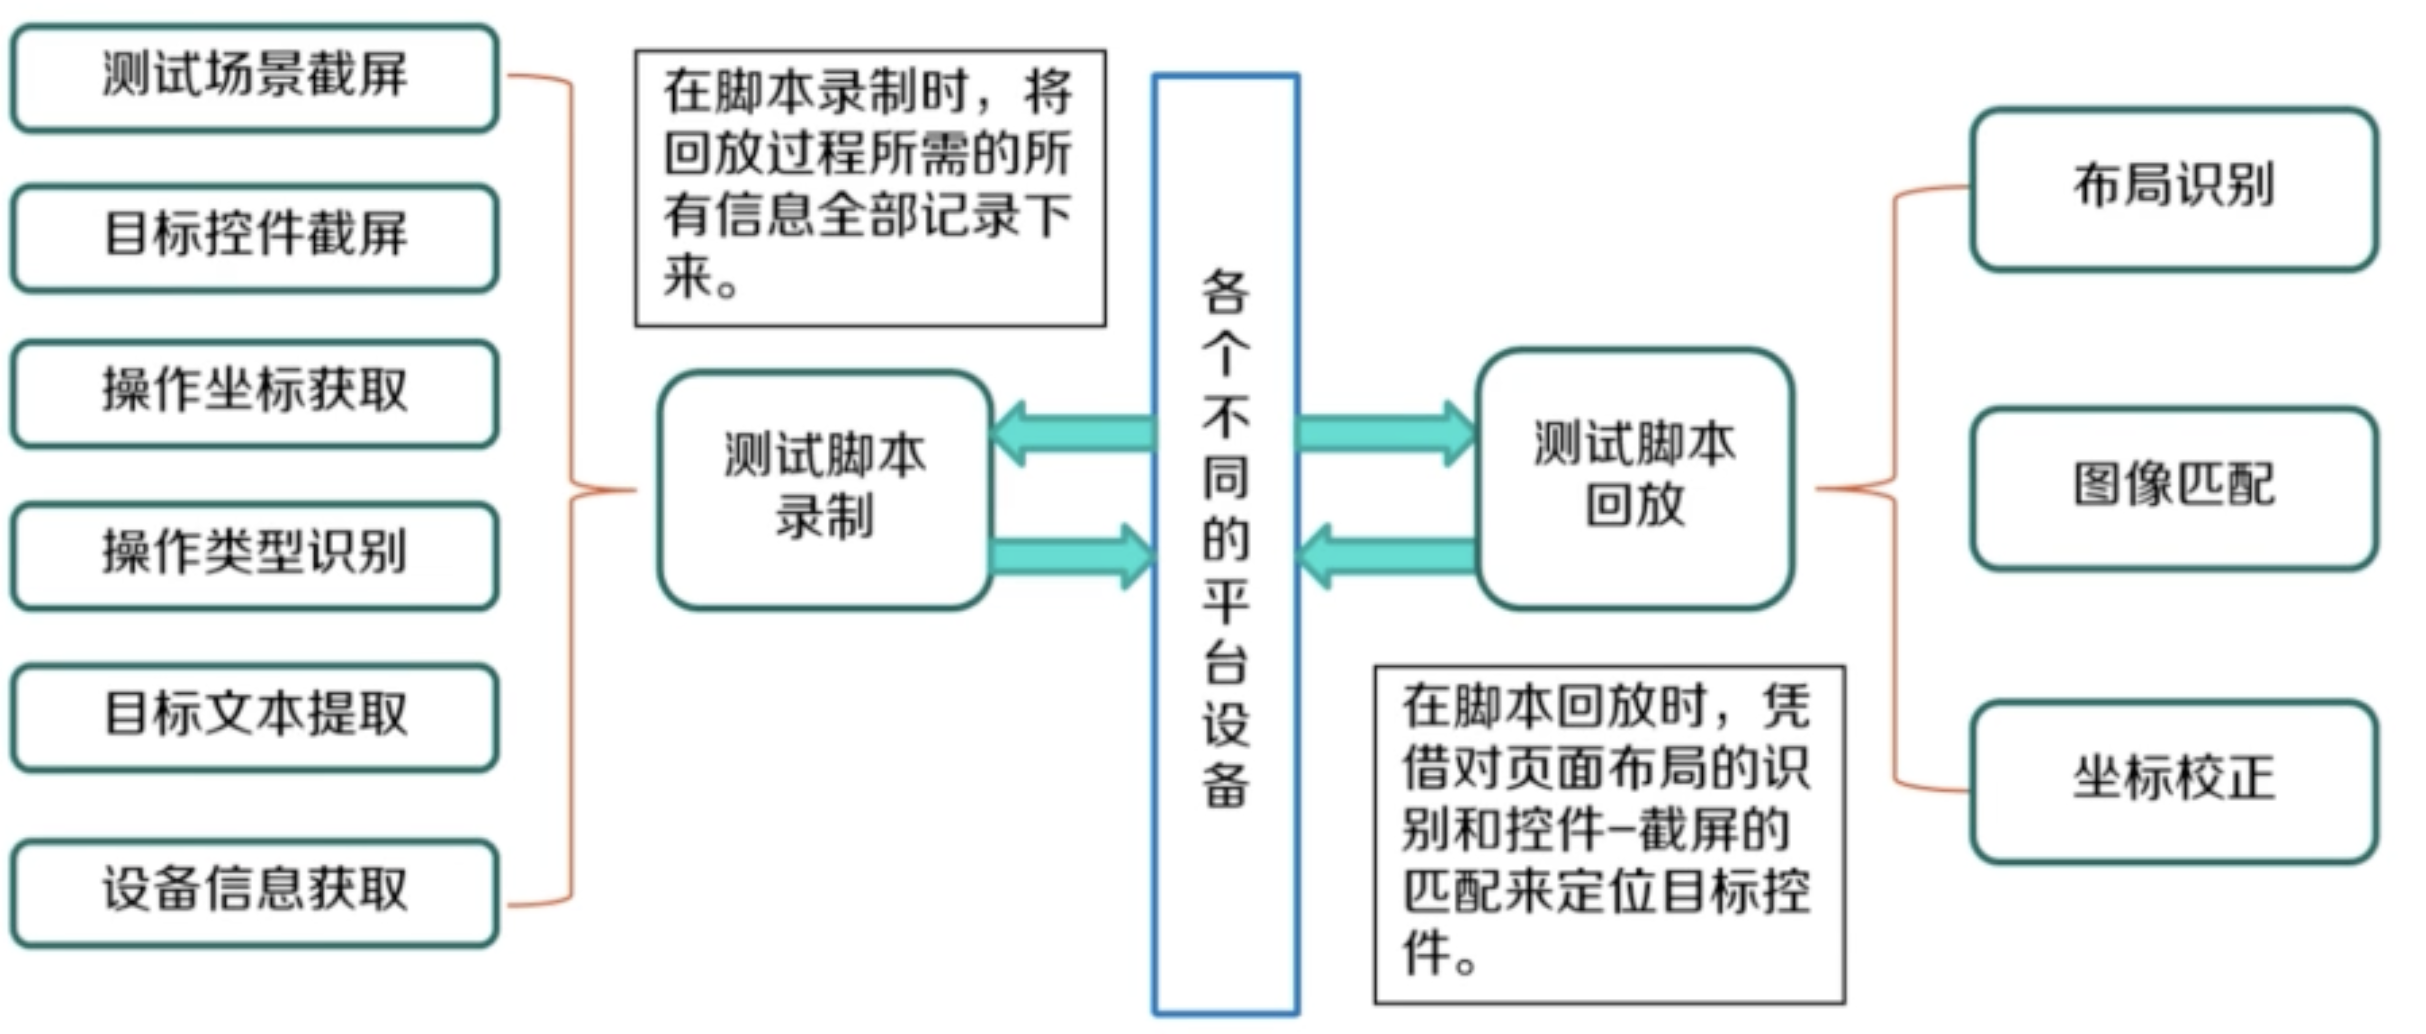
\includegraphics[width=0.8\textwidth]{images/脚本录制与回放的基本框架.png}
    \vspace{-1em}
\end{figure}

\subsection{跨平台的脚本结构}
\begin{figure}[H]
    \vspace{-0.5em}
	\centering
	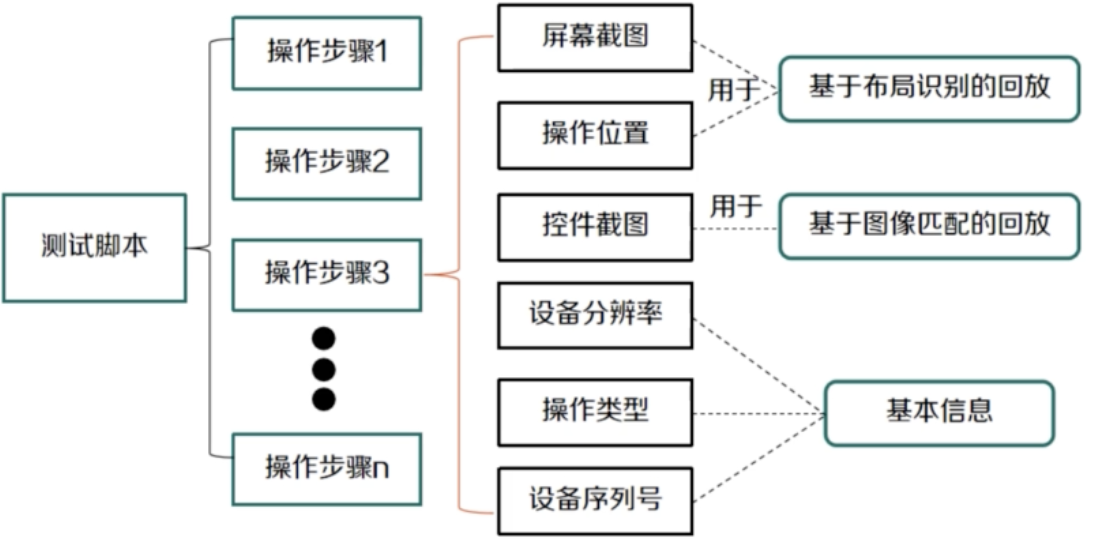
\includegraphics[width=0.7\textwidth]{images/跨平台的脚本结构.png}
    \vspace{-1em}
\end{figure}

\begin{itemize}
    \item 屏幕截图
    \begin{itemize}
        \item \verb|adb shell screencap -p <path>|\ 截屏截图
        \item \verb|adb pull sremote path> <local path>|\ 将手机中的文件\ \verb|<remote path>| \ 拷贝到PC的\ \verb|<local path>|
    \end{itemize}
    \item 控件截图
    \begin{itemize}
        \item \verb|adb shell uiautomator dump <path>|\ 获取界面布局
        \item \verb|adb pull|\ 命令将其拷贝到PC
        \item 利用操作的坐标定位控件,井将其从截图中截取出来
    \end{itemize}
    \item 操作类型、操作位置
    \begin{itemize}
        \item 通过前端JavaScript脚本的各类事件监听器
    \end{itemize}
    \item 设备分辨率、设备序列号
    \begin{itemize}
        \item \verb|AndroidDebugDridge.IDeviceChangeListener|
    \end{itemize}
\end{itemize}

\subsection{脚本的回放}

\subsubsection{图像特征比对}
\begin{figure}[H]
    \vspace{-0.5em}
	\centering
	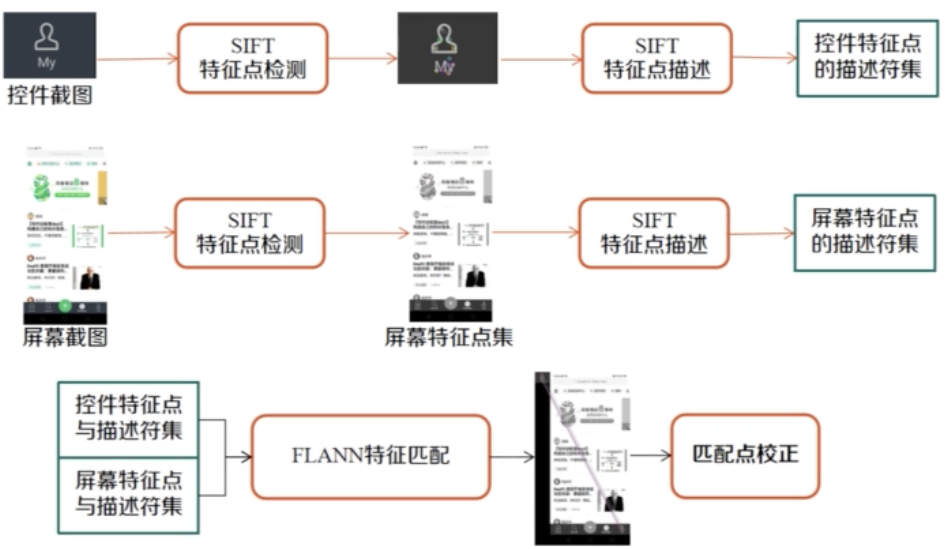
\includegraphics[width=0.8\textwidth]{images/图像特征比对.png}
    \vspace{-1em}
\end{figure}

\subsubsection{布局刻画}
\begin{itemize}
    \item 利用计算机视觉算法从GUI截图中找到所有控件的位置
    \item 利用OCR技术提取GUI截图中的文本
    \item 为所提取出来的控件划分控件组、行和列
\end{itemize}

\begin{figure}[H]
    \vspace{-0.5em}
	\centering
	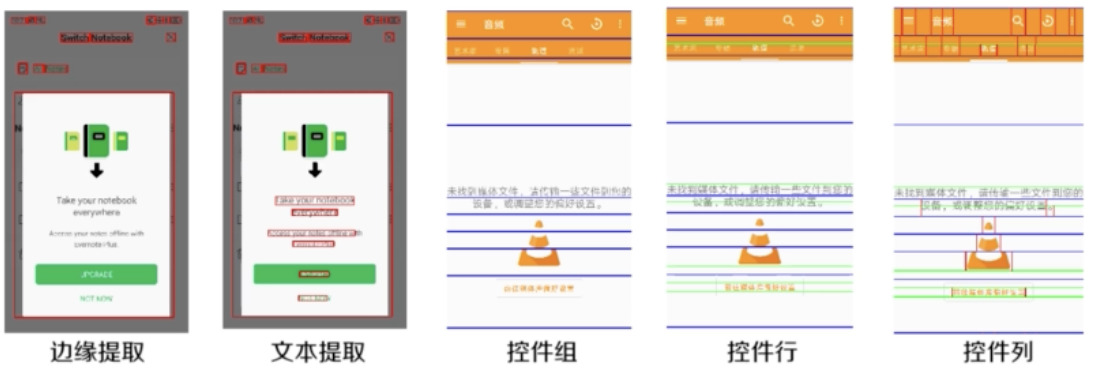
\includegraphics[width=0.85\textwidth]{images/布局刻画.png}
    \vspace{-1em}
\end{figure}

\subsubsection{坐标校正}
\begin{itemize}
    \item 基于布局识别的控件定位
    \begin{itemize}
        \item 容易受不同平台的外部布局的影响
        \item 不易受到图像变化的影响
    \end{itemize}
    \item 基于图像匹配的控件定位
    \begin{itemize}
        \item 容易受到图像变化的影响
        \item 不易受到不同平台的外部布局的影响
    \end{itemize}
    \item 为了结合二者的优点,提升算法的鲁棒性,引入了权重参数$\gamma$
    \begin{itemize}
        \item $W_{final} = \gamma \times W_{layout} + (1-\gamma) \times W_{image}$
        \begin{itemize}
            \item $W_{final}$:最终的控件定位
            \item $W_{layout}$:基于布局识别得到的控件定位
            \item $W_{image}$:基于图像匹配得到的控件定位
        \end{itemize}
    \end{itemize}
\end{itemize}
